\section{A Modelagem da DSL Cotas}
\label{sec:dslproposta:usuario}

   
 Tendo como base a análise realizada no Capítulo \ref{chap:historicoversoes}, sobre as versões do sistema de cotas detalhadas nas Subseções \ref{versao1}, \ref{versao2} e \ref{versao3}, podem ser  pontuadas algumas características em comum identificadas entre cada uma dessas versões:
   
   \begin{enumerate}
    \item[a)] A divisão das vagas entre as diferentes categorias de cotas se deu em formato hierárquico, iniciando no total de vagas o qual foi sendo subdividido em percentuais reservados para suas subcategorias (ex: Estudantes da escola pública, Estudantes com renda baixa, Estudantes PCD, etc); 
   
   \item[b)] Esses percentuais são de conhecimento dos usuários especialistas no sistema de cotas, e podem variar de acordo com a documentação da legislação vigente, ou outras definições que variam conforme a Unidade Federada que oferta o curso; 
   
   \item[c)] Em muitos casos, não é definido um valor de percentual fixo, de modo que uma categoria recebe o valor calculado restante de vagas da categoria pai. Por exemplo, o percentual de cotistas \gls{PCD} é aplicado, e o que resta das vagas vai para candidatos da mesma categoria que não são \gls{PCD};

   \item[d)] Todas as versões consideravam a ordem de prioridade entre as diferentes categorias de cotas passíveis de inscrição;
   
   \item[e)] Questões de arredondamento das vagas (para cima ou para baixo), devem ser consideradas e podem variar de acordo com a versão de lei implementada.

   \end{enumerate}
   
   Segundo \citeonline{dslengineering}, a modelagem de DSLs costuma ser realizada com abordagens \textit{bottom-up} ou \textit{top-down}, a primeira abordagem aplica-se para domínios em termos de software, enquanto na segunda, o modelo do domínio é aplicado ao conhecimento sobre o mundo real, fora do domínio de software. Nesse contexto, a modelagem da DSL Cotas utilizou a abordagem \texttt{top-down}, uma vez que seu design procura fornecer suporte para os usuários especialistas definirem os parâmetros da legislação de forma controlada, possibilitando a geração do código de processamento de classificação de candidatos sem que o usuário precise utilizar comandos complexos para a implementação dos respectivos algoritmos.
   
   A \gls{DSL} desenvolvida consistiu em criar um modelo que permita a configuração de todos os itens listados, tais como: identificador da versão de lei, lista de variáveis para configuração de percentuais, formas de aplicação de arredondamento, uma macro para aplicar a função de resto de vagas de uma categoria, campo descritivo para os diferentes tipos de categorias, estrutura para divisão em subcategorias e lista de ordem de prioridade para a sobra de vagas.
   
   
   
    Na Seção \ref{sec:mps}, são apresentados os componentes desenvolvidos no MPS que são responsáveis pela construção da DSL Cotas.
    
   \section{Componentes da DSL Cotas no \gls{MPS}}
\label{sec:mps}

Nessa Seção são descritos os elementos de modelagem criados na ferramenta \gls{MPS} tais como: os componentes de estrutura (\texttt{structure concepts}), a sintaxe dos editores projecionais (\texttt{editors}), restrições de escopo (\texttt{constraints}), comportamentos de conceitos (\texttt{behaviors}), sistema de tipos (\texttt{typesystem}) e, por fim, os elementos de geração de texto (\texttt{textGen}).

\subsection{\textit{Componentes de estrutura}}
\label{sub:sec:estrutura}

\textit{Concepts} ou conceitos no \gls{MPS} servem para definir a estrutura base da linguagem, cada conceito pode conter propriedades, outros conceitos filhos \texttt{childrens} e referências para outros conceitos. Eles podem herdar ou implementar características de outros conceitos. A Figura \ref{fig:structure} apresenta a lista de conceitos criados para a DSL Cotas.

\begin{figure}[ht!]
\centering

\caption{\textmd{Lista de Conceitos de Estrutura \gls{MPS}}}
\label{fig:structure}
\fcolorbox{gray}{white}{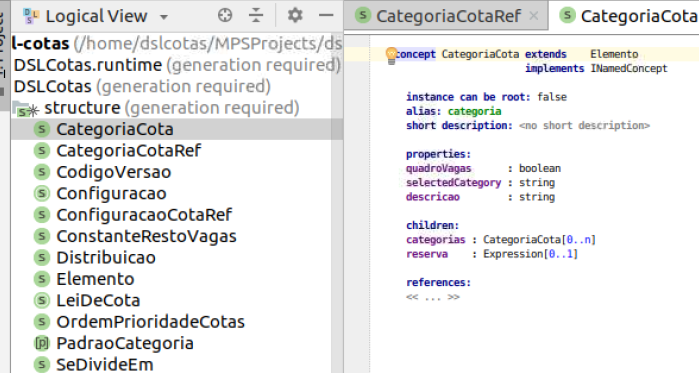
\includegraphics[width=0.70\textwidth]{chapters/dslcotas/mps/imagens/structure.png}}

\par\medskip\textbf{Fonte:} Elaboração do autor (2020) \par\medskip

\end{figure}





Esses conceitos definem a estrutura hierárquica da \gls{AST} de modo análogo ao modelo orientado a objetos, portanto, a Figura \ref{fig:classesmps} mostra a representação da modelagem dos conceitos em formato de diagrama de classes da \gls{UML}.

\begin{figure}[ht!]
\centering

\caption{\textmd{Modelo de Conceitos no \gls{MPS}}}
\label{fig:classesmps}
\fcolorbox{gray}{white}{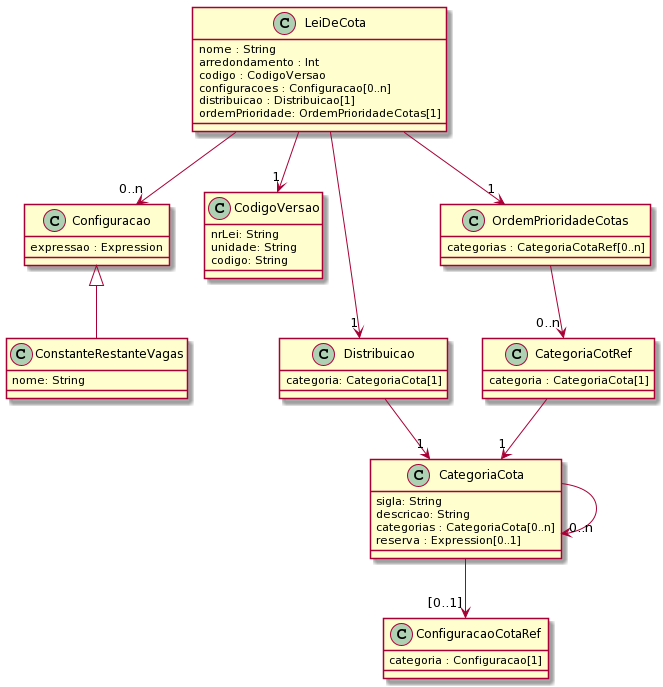
\includegraphics[width=0.70\textwidth]{chapters/dslcotas/mps/imagens/classesmps.png}}

\par\medskip\textbf{Fonte:} Elaborada pelo autor (2020). \par\medskip

\end{figure}




\newpage
O conceito \texttt{LeiDeCota} é o elemento raiz  que pode ser instanciado no \gls{MPS} a fim de criar uma representação abstrata de uma nova lei de cotas na DSL. No \gls{MPS}, os conceitos raiz podem ser criados em módulos \texttt{Solutions}, os quais utilizam uma ou mais linguagens e são os responsáveis por conter o código fonte do usuário final (Figura \ref{fig:solutions}).

\begin{figure}[ht!]
\centering

\caption{\textmd{Criação de elementos raiz em  \texttt{Solutions} no \gls{MPS}}}
\label{fig:solutions}
\fcolorbox{gray}{white}{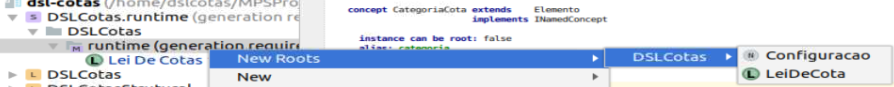
\includegraphics[width=\textwidth]{chapters/dslcotas/mps/imagens/solutions.png}}

\par\medskip\textbf{Fonte:} Elaboração do autor (2020) \par\medskip

\end{figure}



Por sua vez, uma \texttt{LeiDeCota} está associada aos elementos descritos na Tabela \ref{tblelementoslei}:

\begin{table}[ht]
\caption{Elementos associados ao conceito \texttt{LeiDeCota}}
\label{tblelementoslei}
\centering
\begin{tabular}{|p{4.2cm}|p{10cm}|}
\hline
\texttt{CodigoVersao}          & Elemento que mantém informações descritivas sobre a versão de lei aplicada.                                                                                           \\ \hline
Lista de \texttt{Configuracao} & Responsável por armazenar os parâmetros de configuração a serem reutilizados na DSL, contendo o nome da configuração e uma expressão de valor.                          \\ \hline
\texttt{Distribuicao}          & Conceito que contém a \texttt{CategoriaCota} raiz que dará início ao processo de distribuição das vagas entre as suas categorias filhas.                                       \\ \hline
\texttt{OrdemPrioridadeCotas}  & Elemento que contém a lista de referências para as categorias de cotas criadas durante a distribuição e será responsável por manter a ordem de prioridade prevista em lei. \\ \hline
\end{tabular}
  \par\medskip\textbf{Fonte:} Elaborada pelo autor (2020). \par\medskip
\end{table}

   
    

Para possibilitar a relação entre as regras definidas, alguns componentes da \gls{DSL} utilizam \texttt{references} para outros, possibilitando que elementos já definidos possam ser acessados pelos comandos \texttt{control+espaço} no \gls{MPS}. As \texttt{references} são restringidas pelo tipo do conceito alvo e pela cardinalidade, por exemplo, o conceito \texttt{CategoriaCotaRef} possui uma referência para uma \texttt{CategoriaCota} e, por sua vez, o elemento \texttt{OrdemPrioridadeCotas} possui lista de \texttt{CategoriaCotaRef} para que seja possível indicar na linguagem a ordem de prioridade criada durante a distribuição de vagas (Figura \ref{fig:references}).

\begin{figure}[ht!]
\centering

\caption{\textmd{Definição de \texttt{References} no \gls{MPS}}}
\label{fig:references}
\fcolorbox{gray}{white}{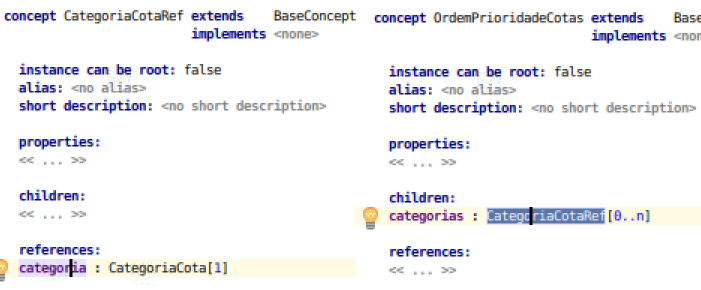
\includegraphics[width=\textwidth]{chapters/dslcotas/mps/imagens/references.png}}

\par\medskip\textbf{Fonte:} Elaborada pelo autor (2020). \par\medskip

\end{figure}



\newpage
Por fim, o conceito \texttt{Distribuicao} é o responsável por armazenar a árvore de distribuição, iniciando com a \texttt{CategoriaCota} raiz, na qual contém uma sigla, uma descrição, uma \texttt{Expression} onde será preenchida a reserva de vaga (percentuais fixos ou itens de \texttt{Configuracao} pré-definidos) e também uma lista de categorias filhas. 

Na Subseção \ref{sub:sec:editores}, serão apresentados os editores criados para definição da sintaxe de cada conceito definido na modelagem.


\subsection{\textit{Editores de conceitos}}
\label{sub:sec:editores}
O \gls{MPS} oferece aos projetistas uma abordagem de definição de sintaxe abstrata por meio de editores construídos com a notação de células. O \textit{designer} da linguagem combina as células do editor e as posiciona de maneira a refletir o layout final desejado da notação \cite{jetbrains}. 

Por padrão os elementos \texttt{Concepts} não possuem um editor associado, o editor padrão permite a edição direta da \gls{AST} pelo usuário da linguagem. No entanto, o editor padrão não é de simples entendimento para os usuários finais da linguagem, sendo necessário definir como aquele conceito deverá ser apresentado e editado pelo usuário.

Nesse sentido a Figura \ref{fig:editors}, apresenta a lista de editores criados para a DSL de cotas. As definições desses editores são apresentadas a seguir.

\begin{figure}[ht!]
\centering

\caption{\textmd{Editores de conceitos da DSL Cotas}}
\label{fig:editors}
\fcolorbox{gray}{white}{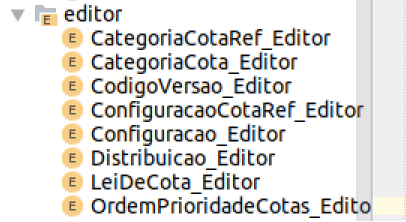
\includegraphics[width=0.85\textwidth]{chapters/dslcotas/mps/imagens/editors.png}}

\par\medskip\textbf{Fonte:} Elaboração do autor (2020) \par\medskip

\end{figure}




O primeiro editor \texttt{LeiDeCota\_Editor} é responsável pela organização das informações relevantes para o modelo de cotas, na Figura \ref{fig:editorleicota} observa-se que ele é composto por uma coleção de células organizadas verticalmente, essa coleção é representada por \texttt{'[-' e '-]'}. Dentro de cada linha da coleção é possível utilizar propriedades básicas do conceito, como por exemplo o campo \texttt{name}. 

\begin{figure}[ht!]
\centering

\caption{\textmd{Editor do conceito LeiDeCota}}
\label{fig:editorleicota}
\fcolorbox{gray}{white}{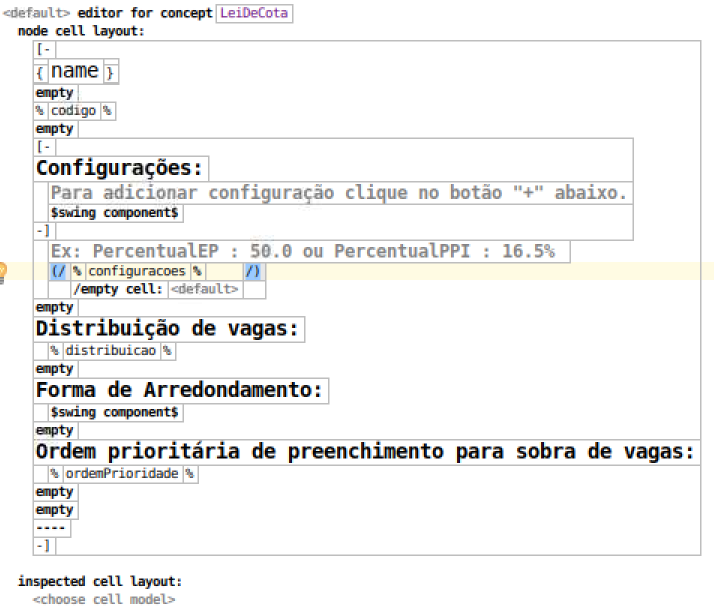
\includegraphics[width=0.85\textwidth]{chapters/dslcotas/mps/imagens/editorleicota.png}}

\par\medskip\textbf{Fonte:} Elaboração do autor (2020) \par\medskip

\end{figure}




\newpage
Também é permitido criar elementos estáticos para descrição de seções, como no caso do texto "Distribuição de Vagas" e referenciar os elementos \texttt{childrens} do conceito, por exemplo, \texttt{\%configuracoes\%}. No entanto, para que os elementos filhos sejam apresentados adequadamente para o usuário é necessário também definir o respectivo editor. 

Por se tratar de um editor de múltiplas projeções, é possível inserir nos editores do \gls{MPS} alguns recursos gráficos disponíveis em sua linguagem base, Java, como por exemplo elementos de \texttt{JTable} e \texttt{JButton} das bibliotecas gráficas \texttt{swing}. A Figura \ref{fig:swingbutton} demonstra um exemplo de como a célula \texttt{\$swing\_component\$} é implementada para inserir o botão de adição de novas configurações na DSL.

\begin{figure}[ht!]
\centering

\caption{\textmd{Exemplo de componente de projeção gráfica}}
\label{fig:swingbutton}
\fcolorbox{gray}{white}{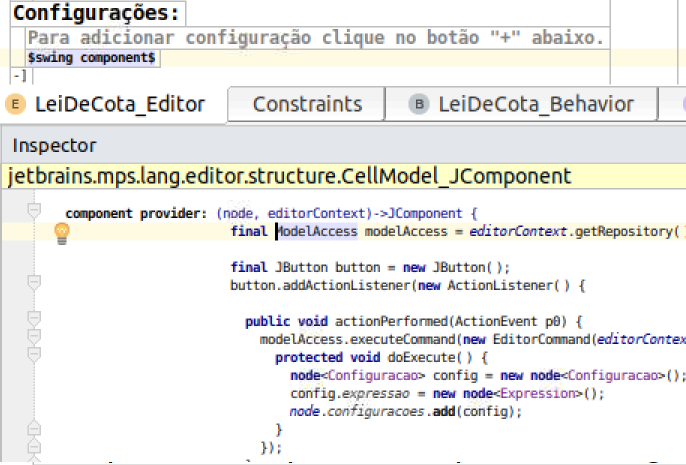
\includegraphics[width=0.75\textwidth]{chapters/dslcotas/mps/imagens/swingbutton.png}}

\par\medskip\textbf{Fonte:} Elaboração do autor (2020) \par\medskip

\end{figure}



Com objetivo de simplificar a edição da árvore de distribuição de vagas para o usuário final da DSL, foi utilizado o recurso \texttt{table} (\texttt{de.slisson.mps.tables}), que se trata de um plugin disponibilizado pelo pacote do \texttt{Mbeddr}\footnote{O Mbeddr é uma coleção de pacotes utilitários e extensões do MPS que permite a criação de muitos tipos diferentes de linguagens no \gls{MPS} \cite{mbeddr}.}. Segundo , as tabelas podem ser usadas para representar coleções de dados estruturados ou apresentar preocupações bidimensionais.

Nesse sentido, na Figura \ref{fig:tableeditor} é possível observar o \texttt{CategoriaCota\_Editor} onde as categorias filhas existentes são renderizadas com esse \textit{plugin} por meio dos comandos \texttt{table\{\}} e \texttt{getHeaders}, onde são iterados todos os seus filhos, de modo que as categorias sejam divididas por linhas indicando a sigla da categoria e o respectivo número de contagem de categorias, resultando no exemplo da Figura \ref{fig:tableeditorres}.

\begin{figure}[ht!]
\centering

\caption{\textmd{Editor com o plugin \texttt{table} do \texttt{Mbeddr}}}
\label{fig:tableeditor}
\fcolorbox{gray}{white}{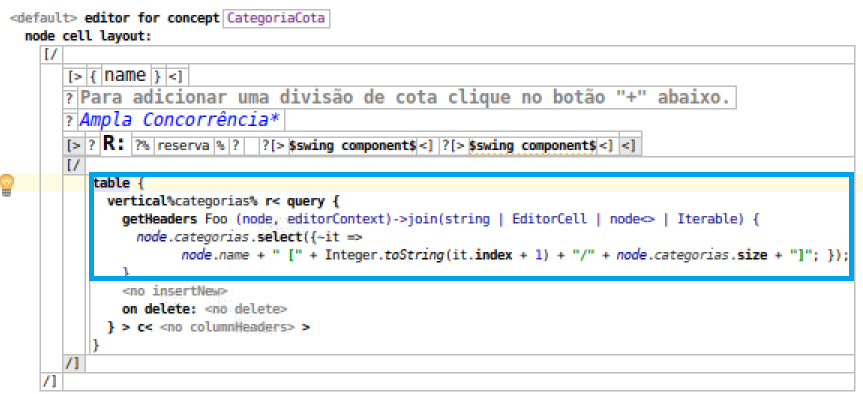
\includegraphics[width=0.95\textwidth]{chapters/dslcotas/mps/imagens/table.png}}

\par\medskip\textbf{Fonte:} Elaboração do autor (2020) \par\medskip

\end{figure}



\begin{figure}[ht!]
\centering

\caption{\textmd{Exemplo de resultado com uso do plugin \texttt{table}}}
\label{fig:tableeditorres}
\fcolorbox{gray}{white}{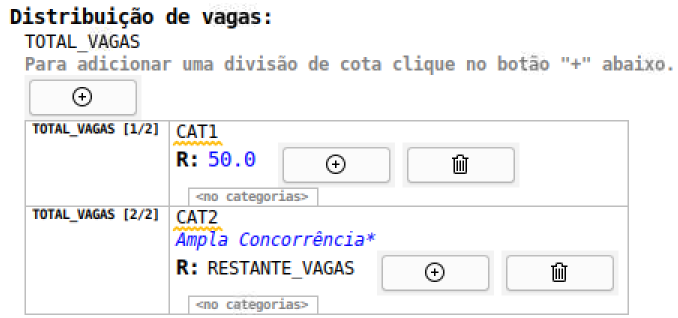
\includegraphics[width=0.95\textwidth]{chapters/dslcotas/mps/imagens/tableres.png}}

\par\medskip\textbf{Fonte:} Elaboração do autor (2020) \par\medskip

\end{figure}



\newpage
Após a definição de editores para todos os conceitos do modelo da linguagem, foi necessário utilizar o recurso de \texttt{constraints} para criar restrições de escopo para acesso às referências entre os elementos da linguagem. Esse detalhamento é observado na Seção \ref{sub:sec:constraints}.

\newpage
\subsection{\textit{Restrições de escopo}}
\label{sub:sec:constraints}

Na presente pesquisa utilizou-se do recurso de restrições de escopo, que se aplica nas restrições de acesso para referências de configurações e categorias de cotas, dentro do contexto de um elemento de \texttt{LeiDeCota} criado pelo usuário da DSL. Possibilitando, por exemplo, que o \gls{MPS} preencha o menu de \textit{code-complete} somente valores válidos para aquela versão da lei de cotas e não mostre opções existentes em  outras versões já definidas.
 
\begin{citacao}
O aspecto de estrutura da linguagem pode ser insuficiente para expressar restrições avançadas para a DSL. O aspecto \texttt{constraints} do MPS fornece uma maneira de definir essas restrições adicionais. Referências dependem da definição de restrições de escopo, já que por padrão quando nenhum escopo é definido para uma referência, essas podem ser utilizadas em qualquer parte da modelagem da linguagem \cite[s/p, tradução nossa]{jetbrains}.
\end{citacao}

Desse modo, nos conceitos de \texttt{CategoriaCotaRef} e \texttt{ConfiguracaoCotaRef} utilizou-se o conceito de definição de escopo herdado ou \textit{inherited scopes} (Figura \ref{fig:scoperef}). Confome \citeonline[s/p, tradução nossa]{jetbrains}, "esse mecanismo delega a resolução do escopo aos ancestrais, que implementam o ScopeProvider".

\begin{figure}[ht!]
\centering

\caption{\textmd{Definição de gerenciador de escopo}}
\label{fig:scoperef}
\fcolorbox{gray}{white}{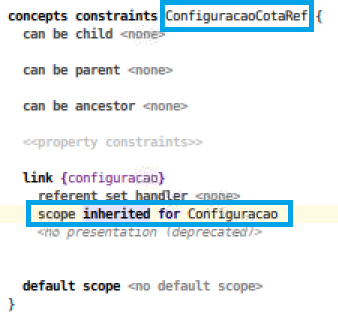
\includegraphics[width=0.55\textwidth]{chapters/dslcotas/mps/imagens/scoperef.png}}

\par\medskip\textbf{Fonte:} Elaborada pelo autor (2020). \par\medskip

\end{figure}



\newpage

Nesse sentido, \gls{MPS} inicia a procura por provedores de escopos nos ancestrais de \texttt{Configuracao} até encontrar algum conceito que sobrescreva a implementação do método \texttt{getScope} da classe \texttt{ScopeProvider} do \gls{MPS}. 

No caso da DSL Cotas o provedor de escopo foi o elemento \texttt{LeiDeCota} (Código Fonte \ref{lst:scopeprovider}), no qual todas as categorias da distribuição e as configurações de cota são adicionadas em uma lista (Linha 13) e retornadas por meio da criação de um \texttt{ListScope} (Linha 16) o qual é retornado sempre que acionado durantes os comandos de \texttt{code-complete} pelo usuário da linguagem (Figura \ref{fig:codecomplete}).

\lstinputlisting[language=Java, 
caption=Implementação do ScopeProvider 
,label=lst:scopeprovider]{chapters/trechos_codigo/scopeprovider.m}

\begin{figure}[ht!]
\centering

\caption{\textmd{\textit{Code-complete}} para referências da \texttt{LeiDeCota}}
\label{fig:codecomplete}
\fcolorbox{gray}{white}{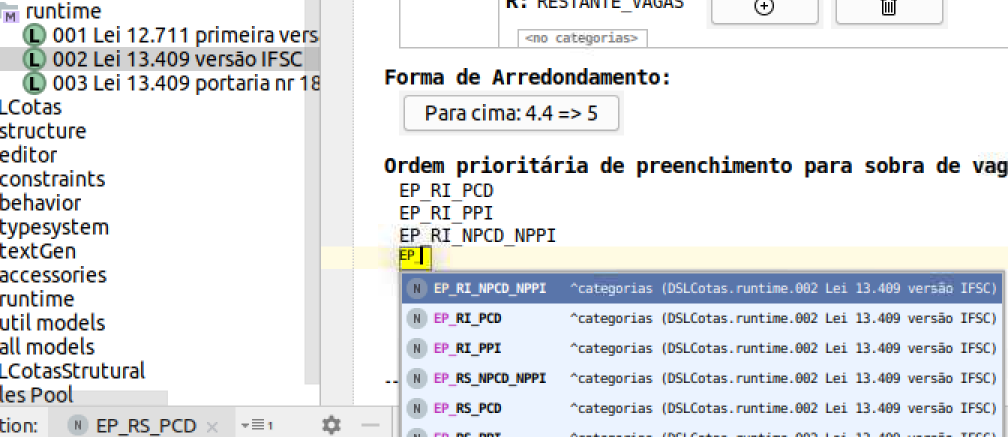
\includegraphics[width=0.95\textwidth]{chapters/dslcotas/mps/imagens/codecomplete.png}}

\par\medskip\textbf{Fonte:} Elaboração do autor (2020) \par\medskip

\end{figure}



Na Seção \ref{sub:sec:comportamentos} é apresentado o aspecto de definição de comportamentos de conceitos (\textit{behaviors}) da DSL Cotas.

\newpage
\subsection{\textit{Comportamento dos elementos de conceito}}
\label{sub:sec:comportamentos}

Durante a manipulação \gls{AST} no \gls{MPS}, operações comuns são frequentemente extraídas para métodos utilitários, a fim de simplificar a tarefa e reutilizar a funcionalidades. O aspecto \textit{behavior} possibilita a criação de métodos de instância, métodos estáticos e construtores de instância dos conceitos \cite{jetbrains}.

Na presente pesquisa, esse aspecto foi utilizado principalmente para simplificar implementações de verificações de inconsistências, fazer validações, implementar operações de \textit{quick fixes} para o usuário da linguagem e também para apoio em questões relacionadas a extração das regras em formato JSON pelo recurso de \texttt{textGen}. A Figura \ref{fig:behaviorlista} apresenta a lista dos \texttt{behaviors} presentes no fonte da DSL Cotas.

\begin{figure}[ht!]
\centering

\caption{\textmd{\texttt{Behaviors da DSL Cotas}}}
\label{fig:behaviorlista}
\fcolorbox{gray}{white}{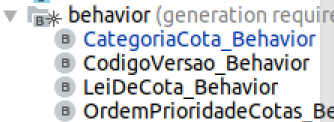
\includegraphics[width=0.60\textwidth]{chapters/dslcotas/mps/imagens/behaviorslista.png}}

\par\medskip\textbf{Fonte:} Elaboração do autor (2020) \par\medskip

\end{figure}



Um exemplo de \texttt{concept behavior} é apresentado na Figura \ref{fig:behaviorcat}, para o conceito \texttt{CategoriaCota}, onde o método \texttt{isClag}, responsável por verificar se a categoria corrente é a categoria correspondente à ampla concorrência, possibilitando distingui-la e informar ao usuário o respectivo ramo na distribuição onde ela deve ser definida (Figura \ref{fig:behaviorcatuso}).

\begin{figure}[ht!]
\centering

\caption{\textmd{Exemplo de \textit{concept behavior} para \texttt{CategoriaCota}}}
\label{fig:behaviorcat}
\fcolorbox{gray}{white}{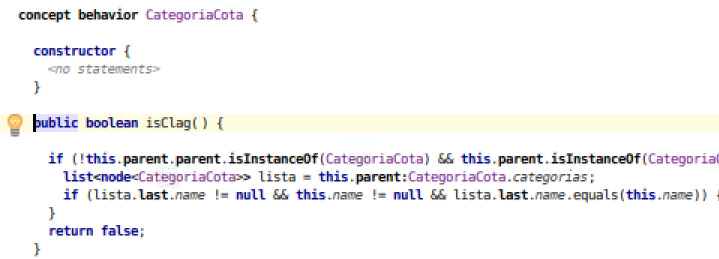
\includegraphics[width=0.95\textwidth]{chapters/dslcotas/mps/imagens/behaviorCategoria.png}}

\par\medskip\textbf{Fonte:} Elaborada pelo autor (2020). \par\medskip

\end{figure}



\begin{figure}[ht!]
\centering

\caption{\textmd{Uso do método \texttt{isClag} para identificar nível de Ampla Concorrência}}
\label{fig:behaviorcatuso}
\fcolorbox{gray}{white}{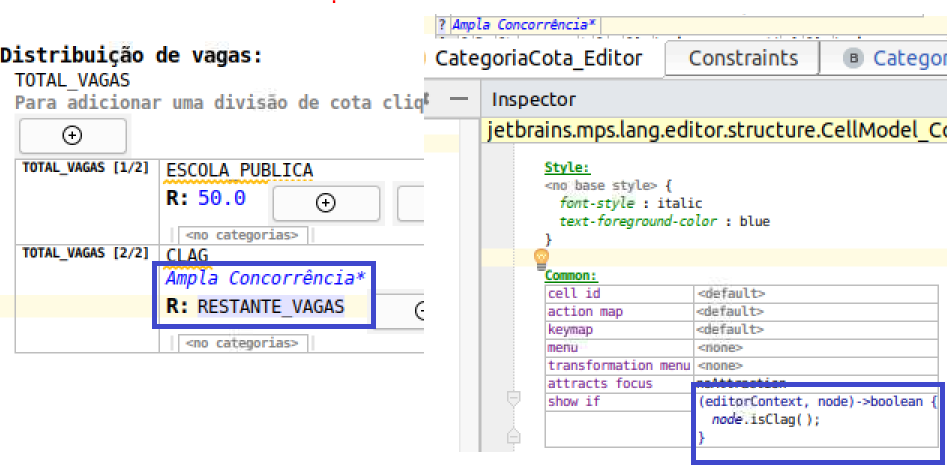
\includegraphics[width=0.85\textwidth]{chapters/dslcotas/mps/imagens/behaviorCategoriauso.png}}

\par\medskip\textbf{Fonte:} Elaboração do autor (2020) \par\medskip

\end{figure}



Em continuação ao objetivo de descrever os recursos que fornecem apoio aos usuários da linguagem, a Seção \ref{sub:sec:typesystem} apresenta o sistema de tipos criado para a DSL Cotas, o qual possibilita a definição controlada das regras de cotas para o usuário final.

\subsection{\textit{Sistema de tipos}}
\label{sub:sec:typesystem}

Segundo \citeonline{campagne2014mps}, o aspecto \textit{typesystem} do \gls{MPS} é um componente da linguagem que torna possível calcular tipos da \gls{AST} e também serve para definir e reportar erros de semântica para o usuário da linguagem. Nesse sentido, são descritos os seguintes conceitos utilizados na DSL, conforme documentação do \gls{MPS} \citeonline{jetbrains}:

\begin{enumerate}
 
 \item[a)] \texttt{Checking rules}: São regras de verificação que podem realizar uma busca no modelo à procura de padrões de erros conhecidos no código e relatá-los ao usuário, também são conhecidas como análise estática de código. O \gls{MPS} diferencia os problemas conforme a severidade: \textit{erros}, \textit{warning} e \textit{infos}, respectivamente, por meio de destaques nas cores vermelha, amarela e cinza;
 
 \item[b)]\texttt{Quick Fix}: São responsáveis por implementar correções automáticas, fornecendo uma função de transformação do modelo, eliminando o problema relatado para o usuário. Por exemplo, um quick fix poderia ser criado para eliminar automaticamente trechos de código ou declarações duplicadas;
 
 \item[c)]\texttt{Inference Rules}: Uma regra de inferência para um determinado \textit{concept} é responsável principalmente por computar um tipo para instâncias desse conceito. O \gls{MPS} fornece uma série de métodos de inferência, tais como: expressões de \textit{typeof}, declarações \textit{when concrete}, \textit{equations} e \textit{inequations}, etc. Esses recursos podem ser utilizados, por exemplo, para verificar se o tipo de uma variável local é igual ao tipo da sua declaração.
\end{enumerate}


A Tabela \ref{tblcheckingrules}, apresenta a lista de \texttt{checking rules} implementadas na DSL Cotas, enquanto a Tabela \ref{tblquickfixes}, elenca os elementos de \texttt{quick fixes} implementados como recursos de apoio ao usuário.


\begin{table}[ht]
\caption{\textit{Checking rules} da DSL Cotas}
\label{tblcheckingrules}
\centering

\begin{tabular}{|p{6cm}|p{8cm}|}
\hline
\texttt{categoria\_resestante\_vagas} & Busca identificar se o último ramo de uma divisão de vagas é preenchida pelo usuário com a constante \texttt{RESTANTE\_VAGAS}.                                                                                      \\ \hline
\texttt{categoria\_unica} & Impede siglas de categorias de cotas duplicadas.                         \\ \hline
\texttt{codigo\_versao\_lei}          & Valida padrões de preenchimento dos dados de identificação da lei de cotas.                                       \\ \hline
\texttt{configuracao\_simples}          & Impede que o usuário preencha expressões complexas em uma definição do conceito \texttt{Configuracao}.
                        \\ \hline
\texttt{divisao\_pelo\_menos\_dois\_ramos}          & Garante que uma divisão de categoria possua pelo menos 2 (duas) categorias, exceto o ramo raiz.
                        \\ \hline
\texttt{filha\_sem\_reserva}          & Verifica se todas as categorias possuem o campo de percentual de reserva preenchido.

\\ \hline
               
\texttt{formato\_sigla\_cota}          & Faz o \textit{matching} da \texttt{String} de siglas de cota, permitindo apenas caracteres alfanuméricos maiúsculos.
\\ \hline

\texttt{distribuicao\_nome}          & Garante que o ramo raiz \texttt{TOTAL\_VAGAS} não tenha o nome alterado pelo usuário da DSL.
\\ \hline

\texttt{ordem\_prioridade\_duplicada}          & Valida se o usuário informou uma categoria de cota duplicada no conceito \texttt{OrdemPrioridadeCotas}.
\\ \hline

\texttt{ordem\_prioridade\_catfilhas}          & Gera um \textit{warning} para o usuário quando uma categoria não foi informada na seção \texttt{OrdemPrioridadeCotas}.
\\ \hline

\texttt{warning\_nm\_inic\_cota}          & Sugere um nome de preenchimento para a sigla de cota que inicie com o prefixo da cota anterior, por exemplo: a cota de estudantes de renda inferior (sigla RI), que fica dentro da categoria de escola pública (sigla EP), tem como sugestão EP\_RI, para facilitar a identificação.
\\ \hline

\end{tabular}

  \par\medskip\textbf{Fonte:} Elaborada pelo autor (2020). \par\medskip
\end{table}

\newpage
\begin{table}[ht]
\caption{\textit{Quick fixes da DSL Cotas}}
\label{tblquickfixes}
\centering

\begin{tabular}{|p{6cm}|p{9cm}|}
\hline
\texttt{preenche\_totalvagas\_name} & \textit{Quick fix} associado ao erro gerado pela \textit{checking rule} \texttt{distribuicao\_nome}, faz o preenchimento automático do nome padrão no ramo raiz de distribuição de vagas.                                                                                      \\ \hline
\texttt{remover\_categoria\_duplicada} & \textit{Quick fix} associado ao erro gerado pela \textit{checking rule} \texttt{categoria\_unica}, sugere a remoção automática do ramo de distribuição com a duplicidade.

\\ \hline
\texttt{reserva\_vagas\_ultima\_da\_lista} & \textit{Quick fix} associado ao erro gerado pela \textit{checking rule} \texttt{categoria\_resestante\_vagas}, sugere a correção automática da distribuição de vagas para preenchimento adequado da constante \texttt{RESTANTE\_VAGAS}.

\\ \hline
\texttt{sugere\_sigla\_nome} & \textit{Quick fix} associado ao \textit{warning} gerado pela \textit{checking rule} \texttt{warning\_nm\_inic\_cota}, sugerindo a correção automática para padronização do nome das siglas de distribuição.
                  \\ \hline      

\end{tabular}

  \par\medskip\textbf{Fonte:} Elaboração do autor (2020) \par\medskip
\end{table}




Com relação aos recursos de regras de inferência (\textit{inference rules}), foram definidas as regras: \texttt{typeof\_CategoriaCota} e \texttt{typeof\_Configuracao}, criadas para verificar se os valores dos percentuais são preenchidos somente com expressões ou referências do tipo \texttt{double}.

As Figuras \ref{fig:checkingrule}, \ref{fig:quickfix} e \ref{fig:inferencerule}, demonstram exemplos de como foram implementadas, respectivamente, as \textit{checking rules}, as \textit{quick fixes} e as \textit{inference rules}. 



\begin{figure}[ht!]
\centering

\caption{\textmd{Exemplo de \textit{checking rule}}}
\label{fig:checkingrule}
\fcolorbox{gray}{white}{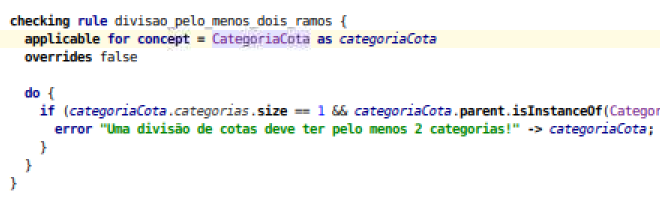
\includegraphics[width=0.85\textwidth]{chapters/dslcotas/mps/imagens/chekingrules.png}}

\par\medskip\textbf{Fonte:} Elaborada pelo autor (2020). \par\medskip

\end{figure}


\begin{figure}[ht!]
\centering

\caption{\textmd{Exemplo de \textit{quick fix}}}
\label{fig:quickfix}
\fcolorbox{gray}{white}{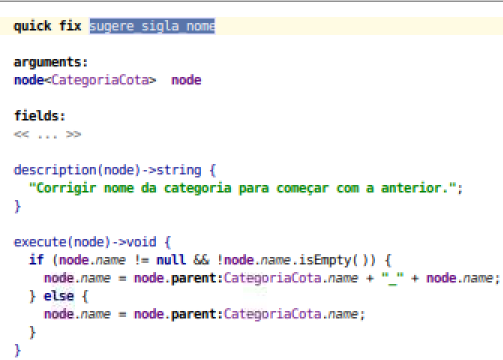
\includegraphics[width=0.85\textwidth]{chapters/dslcotas/mps/imagens/quickfixes.png}}

\par\medskip\textbf{Fonte:} Elaborada pelo autor (2020). \par\medskip

\end{figure}

\begin{figure}[ht!]
\centering

\caption{\textmd{Exemplo de \textit{inference rule}}}
\label{fig:inferencerule}
\fcolorbox{gray}{white}{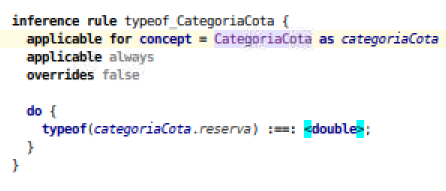
\includegraphics[width=0.85\textwidth]{chapters/dslcotas/mps/imagens/inferencerule.png}}

\par\medskip\textbf{Fonte:} Elaborada pelo autor (2020). \par\medskip

\end{figure}


\newpage
A \textit{checking rule} \texttt{divisao\_pelo\_menos\_dois\_ramos} é aplicada ao conceito \texttt{CategoriaCota} de modo a identificar se o usuário definiu pelo menos 2 (dois) ramos para a sua subdivisão, gerando um erro que é associado ao respectivo ramo da AST com problema (Figura \ref{fig:checkingrule}). Uma \textit{checking rule} pode ser associada a um \textit{quick fix} com objetivo de sugerir correções para o usuário da \gls{DSL}, a exemplo o \textit{quick fix} \texttt{sugere\_sigla\_nome} faz a correção para que as siglas sejam identificadas conforme a sigla da categoria anterior, por exemplo ''EP\_''RI como subcategoria da conta EP (Figura \ref{fig:quickfix}). Por fim, a \textit{inference rule} \texttt{typeof\_CategoriaCota} garante que o campo de reserva seja preenchido com valores e configurações definidas com o tipo \texttt{double} (Figura \ref{fig:inferencerule}).


\newpage
\subsection{\textit{Gerador textGen}}
\label{sub:sec:texgen}

Na presente pesquisa optou-se por implementar o código fonte de classificação de candidatos em formato de \gls{API} externa ao \gls{MPS}, por meio de leitura das definições da DSL Cotas e posterior extração em formato JSON. Isso foi possível mediante o uso do aspecto de \texttt{TextGen} do MPS.

O aspecto de \texttt{TextGen} do MPS define como o modelo da linguagem pode ser transformado em formato textual. Esse recurso é útil sempre que o modelo definido no MPS precise ser convertido diretamente para formato textual \cite{jetbrains}. 

Para tanto, esse recurso requer que cada conceito do modelo seja criado um \textit{text gen component}, onde devem ser utilizadas operações do tipo \textit{append}, para que as informações sejam extraídas no formato texto desejado. Um exemplo da geração do conceito \texttt{CategoriaCota} pode ser observado na Figura \ref{fig:texgen}.

\begin{figure}[ht!]
\centering

\caption{\textmd{Geração do conceito \texttt{CategoriaCota} utilizando \texttt{TextGen}}}
\label{fig:texgen}
\fcolorbox{gray}{white}{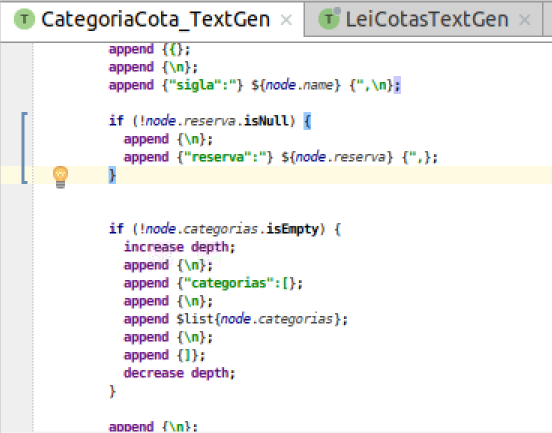
\includegraphics[width=0.85\textwidth]{chapters/dslcotas/mps/imagens/textgen.png}}

\par\medskip\textbf{Fonte:} Elaborada pelo autor (2020). \par\medskip

\end{figure}




Por fim, todos esses componentes permitiram a construção da estrutura necessária para modelagem das regras do sistema de cotas por usuários não desenvolvedores. Em continuidade ao presente estudo, a Subseção \ref{apicotas} detalha a \gls{API} construída com o propósito validar os objetivos que concernem à geração do código fonte de classificação e aprovação de candidatos.

\newpage
